\documentclass[12pt,doublespacing,a4paper]{ouparticle}

%\usepackage[scaled]{helvet}
%\renewcommand\familydefault{\sfdefault} 
%\usepackage[T1]{fontenc}


\usepackage[authoryear]{natbib}
\usepackage{lineno}
\usepackage{pdfpages}
\usepackage{lscape}


\begin{document}

\title{An Example of Conducting Management Strategy Evaluation Using Machine Learning to Evaluate Trade-offs Between Multiple Management Objectives}

\author{%
\name{Laurence T. Kell}
%\address{Centre for Environmental Policy, Imperial College London, London SW7 1NE}\email{e-mail Lauriel@seapluslus.co.uk}
\name{Co\'il\'in Minto}
%\address{GMIT}
\name{Hans Gerritsen}
%\address{Marine Institute}
\name{Alexander J. M. Kell}
}

\abstract{
An example of conducting Management Strategy Evaluation (MSE) using machine learning to evaluate trade-offs between management objectives using an Operating Model conditioned on life history characteristics to evaluate an empirical Harvest Control Rule. The specific aims of the study are to
 \begin{itemize}
  \item  Develop a risk based framework, where is risk is an uncertainty that matters and what matters are management objectives.
  \item  Develop a way of tuning Management Procedures so that case specific management strategies can be developed efficiently.
  \item  Allow stakeholders to more easily agree management objectives and to evaluate the trade-offs between them.
 \end{itemize}
}

\date{\today}

\keywords{}
 
\maketitle

\newpage


\linenumbers
\linespread{2}


\section{Introduction}

The adoption of the precautionary approach \citep[PA,][]{garcia1996precautionary} requires fisheries management to deal explicitly with uncertainty in order to reduce risks to resources, the environment, fishing communities and society. To do this requires the development of robust control rules that function correctly despite the presence of uncertainty \citep{radatz1990ieee, zhou1996robust}. There are many important process, however, about which there is little infomation in datasets used to monitor, assess and control fish stocks  \citep[e.g.][]{bjoernstad2004trends, botsford}.  

There has been a trend towards using stock assessment models of increasing complexity \citep[e.g][]{}, which has led to two problems including a lack of transparency because of many internal, inexplicit and often poorly documented assumptions and a lack of access, as only a few highly skilled modellers can run such complex models \citep{hilborn2003state}.  An alternative approach is to use Management Strategy Evaluation (MSE) to evaluate management decisions based on simple rules that can be data rather than model-based. The rules can be black boxes (with no knowledge of the system dynamics) and act as feedback controllers. Empirical rules based on data work like a thermostat which is able to keep the state of the system within agreed bounds despite being unaware of the internal structure of the system. 

We conduct MSE using an Operating Model (OM) conditioned on life history characteristics which is able evaluate the impact of alternative hypotheses related to population processes. We then evaluate a Management Procedure (MP) based on an emprical HCR where catches are increased when the trend in an index of abundance is positive, and decreased if the trend is negative. 

The aims of the study are to provide a worked example of how to
 \begin{itemize}
  \item  Develop a risk based framework for conducting MSE,  where is risk is an uncertainty that matters and what matters are management objectives.
  \item  Develop an efficient way of tuning Management Procedures so that case specific management strategies can be developed.
  \item  Explore multiple conficting objectives using Pareto-optimal solutions.
  \item  Allow stakeholders to more easily agree management objectives and the trade-offs between them when conducting M
 \end{itemize}


\section{Material and Methods}

The OM was conditioned on life history parameters for turbot, a scenarios was simulated for an increasing trend in fishing mortality ($F$) that leads to overfishing, then a recovery plan is implemented to bring fishing back to the $F_{MSY}$ level. An index of abundance was simulated using an Observation Error Model (OEM).


\subsection{Methods}

The  Operating Model (OM) was conditioning on turbot life history characteristics.  Life history parameters were used to parameterise a \cite{vonbert1957quantitative} growth curve, a logistic ogive for proportion mature-at-age ogive, natural mortality-at-age \citep{lorenzen2002density} and a \cite{beverton1993dynamics} stock recruit relationship. Spawning stock biomass (SSB) was was used as a proxy for stock reproductive potential \citep[SRP][]{trippel_estimation_1999,Trippel 1999,tomkiewicz2003avaliable}. This assumes that fecundity is proportional to the mass-at-age of the sexually mature portion of the population irrespective of the demographic composition of adults \citep{murawski_impacts_2001} and that processes such as sexual maturity are simple functions of age \citep{matsuda_inconsistency_1996} and independent of gender.

These processes allow an equilibrium per-recruit model to be parameterised, which when combined with a stock recruitment relationship \cite{sissenwine1987alternative} is then used to condition a forward projection model to simulate the time series.


\subsubsection{HCR}

The HCR was based on that of the Commission for the Conservation of Southern Bluefin Tuna (CCSBT) which has several parameters that require tuning; i.e. the “best” parameters are found by choosing  values that optimises the outcomes. Where the optimal outcomes depend on the objectives of  asset and stakeholders. 

The Management Procedure (MP) was based on an emprical HCR where catches are increased when the trend in an index of abundance is positive, alternatively catches are decreased if the trend is negative, namely 

\begin{equation}
 TAC^1_{y+1}=TAC_y\times 
 \left\{\begin{array}{rcl}  
    {1-k_1|\lambda|^{\gamma}} & \mbox{for} & \lambda<0\\[0.35cm]
    {1+k_2\lambda} & \mbox{for} & \lambda\geq 0 
 \end{array}\right.
\end{equation}

where $\lambda$ is the slope in the regression of $\ln I_y$ against year for the most recent $n$ years and $k_1$ and $k_2$ are \textit{gain} parameters and $\gamma$ actions asymmetry so that decreases in the index do not result in the same relative change as as an increase.

The TAC is then the average of the last TAC and the value output by the HCR. 

\begin{equation} 
     TAC_{y+1} = 0.5\times\left(TAC_y+C^{\rm targ}_y\right)\\
\end{equation}

An empirical MP has to be tuned, i.e. run for a range of control parameters values ($k_1$,$k_2$, $\gamma$ and $\lambda$) which are then chosen based on the performance of the MP, i.e. the MP that best meets the management objectives is selected. There are trade-offs between the multiple objectives, however, and  deciding which is a "best" MP requires an iterative process involving between managers, stakeholders and scientists.  

Once the objectives are agreed the traditional way to find the control parameters is to perform an exhaustive search through a manually specified set of control parameters, i.e. a grid search. Even for a limited number of control parameters this can take a substantial amount of computing time, a more efficient approach is to use random search where the control parameters are selected from all the potential combinations at random.

\section{Parameter Tuning}

Many real-world problems naturally have multiple objectives to optimise. Traditionally, optimisation methods address this issue by combining multiple objectives into a single-objective, i.e a reward or utility function. This does not, however, take into account the various trade-offs between equally optimal solutions (Pareto-optimal). Or the different objectives of different groups such as fishers, managers, policy makers, consumers and scientists. This makes it important to explore multiple Pareto-optimal solutions. Where a Pareto frontier is made up of many Pareto-optimal solutions. These can be displayed graphically, allowing a stakeholders to choose between various solutions and their trade-offs.

Multi-objective optimization has been used in many different fields, as diverse as ship hull design \cite{Guha2015}, electoral zone planning \cite{Ponsich2017} and energy consumption and indoor environment thermal performance \cite{Yu2015a}. Many such multi-objective problems have been solved with Non-Dominated Sorting Genetic Algorithm II (NSGA-II) \cite{Valkanas2014} and Multi-Objective Genetic Algorithms \cite{T.MurataandH.Ishibuchi1995}. Where objective functions are not smooth evolutionary these techniques have been found to be the most practical and able to determine the global minima in most trials.

Classical methods require multiple applications of an optimization algorithm, with various scalings between rewards to achieve a single reward. The population approach of genetic algorithms, however, enable the Pareto frontier to be found in relatively few simulation runs.

\subsubsection{Genetic Algorithms}
GAs~\cite{Holland1975} are a class of evolutionary algorithms. We detail the workings of genetic algorithms in this section.

An initial population of structures $P_{0}$, for generation 0, is generated and each individual is evaluated for fitness. A subset of individuals, $C_{t+1} \subset P_{t}$, are chosen for mating, selected proportional to their fitness. `Fitter' individuals have a higher chance of reproducing to create the offspring group $C'_{t+1}$. $C'_{t+1}$ have characteristics dependent on the genetic operators: crossover and mutation. The genetic operators are an implementation decision \cite{FogelDavidB2009}. 

Once the new population has been created, the new population $P_{t+1}$ is created by merging individuals from $C'_{t+1}$ and $P_{t}$. See Algorithm \ref{genetic-algorithm} for detailed pseudocode.


NSGA-II is efficient for multi-objective optimization on a number of benchmark problems and finds a better spread of solutions than Pareto Archived Evolution Strategy (PAES)~\cite{Knowles1999} and Strength Pareto EA (SPEA)~\cite{Zitzler2006} when approximating the true Pareto-optimal front \cite{Valkanas2014}.

The majority of multi-objective optimization algorithms use the concept of \emph{domination} during population selection \cite{Burke2014}. A non-dominated genetic algorithm seeks to achieve the Pareto-optimal solution, so no single optimization solution should dominate another. An individual solution $\mathbf{x}^{1}$ is said to dominate another $\mathbf{x}^{2}$, if and only if there is no objective of $\mathbf{x}^{1}$ that is worse than objective of $\mathbf{x}^{2}$ and at least one objective of $\mathbf{x}^{1}$ is better than the same objective of $\mathbf{x}^{2}$ \cite{Bao2017}. Non-domination sorting is the process of finding a set of solutions which do not dominate each other and make up the Pareto front. A Pareto front contains solutions that have dominated all inferior solutions, and have at least one objective which is better than the other solutions of the Pareto front. See Figure \ref{fig:pareto-layering}a for a visual representation, where $f_1$ and $f_2$ are two objectives to minimise.


\section{Results}


Figure 1 shows the trade-off between yield (Yield:MSY) and safety (the minimum expected recruitment relative ) are shown for the individual management strategy evaluations (blue) along with the pareto frontier (red).
Figures 2 show the calibration curves for the control parameters  and  obtained from the pareto frontier for safety, yield and AAV in yield respectively. For a given level of a management objective the corresponding control value can be read off from the Y-axes. The scatter of points reflects that the Pareto frontiers are actually hyperdimensional surfaces projected into 2 dimensions.
The MSE was then run for the control parameters for 2 scenarios corresponding to the CV (10%, 20% and 30%) of the index (x-axis) and the number of years (3, 5, and 7 column) used to estimate the trend in the index  and the summary statistics by scenario are shown in Figure 3.
An objective of the approach is to develop a risk based framework for conducting MSE, where is risk is an uncertainty that matters and what matters are management objectives.  The framework allows asset and stake holders to more easily agree management objectives and the trade-offs between them when conducting MSE. In addition the framework provides an efficient way of tuning Management Procedures so that case specific management strategies can be developed.
The approached used demonstrates a potential stepwise procedure for conducting MSE namely
First a single MSE is run using random search and the Pareto frontiers constructed
Based on this the main objectives and their trade-offs can be elicited from asset and stakeholders
Using the Pareto frontiers the control parameters can be derived by calibration.
Next a set of robustness trials, i.e. for an agreed set of OM that reflect the main uncertainties can be developed and the corresponding Pareto frontiers derived.
A final set of control parameters can then be agreed following dialogue with asset and stakeholders



Figure 3. Summary statistics from MSE.

Figure \ref{fig:om} 
Figure \ref{fig:pareto} 
Figure \ref{fig:control} 
Figure \ref{fig:mse} 
Figure \ref{fig:om} 


\section{Discussion}


\begin{description}
 \item[Uncertainty]  
 \item[Risk]     
 \item[Management Frameworks] 
 \item[Robustness]
 \item[Lessons for data poor case studies]  
 \item[Lessons for data rich case studies] 
\end{description}

%For risks to be managed in a consistent way given the range of uncertainties across data rich and poor stocks requires OMs to be condition on appropriate processes. This allows an evaluation of the relative value-of-information and the value-of-control. In the former case this involves demonstrating the benefit of obtain better knowledge and data, i.e. to move a stock between categories, and in the later to consider alternative forms of indicators and control rules to develop robust advice. ROC curves are related in a direct and natural way to a cost/benefit analysis of diagnostic decision making, i.e. can be used to identify the value of control

%Setting of appropriate reference levels in the f and b component of the rules, and the extent to which this could be done with tuning that depends on life-history traits and/or the nature of the time-series was addressed using tools developed under the MyDas project. The aim of MyDas is to develop and test a range of assessment models and methods to establish Maximum Sustainable Yield (MSY), or proxy MSY reference points across the spectrum of data-limited stocks. To tune a catch rule of the form r f b, requires selecting indicators and reference points for each of the r and b components and then finding multipliers and thresholds for the component in order to combine them into a single rule. Doing this on a stock specific basis can take considerable time using MSE alone, especially as a variety of indicators and reference points can be used.  Therefore an example was developed using a Receiver Operating Characteristic or ROC curve, to show how potential indicators and reference points can be screened for a range of uncertainties before conducting MSE. 


\section{Conclusions}

\begin{itemize}
 \item 
 \item 
 \item 
 \item 
\end{itemize}

\section{Acknowledgement}

Laurence Kell's involvement was funded through the MyDas project under the Marine Biodiversity Scheme which is financed by the Irish government and the European Maritime and Fisheries Fund (EMFF) as part of the EMFF Operational Programme for 2014-2020. 

\clearpage
\bibliography{/home/laurence/Desktop/refs.bib}
\bibliographystyle{apalike}


\clearpage
\section{Figures}

\newpage
\begin{figure}[h]
\centering
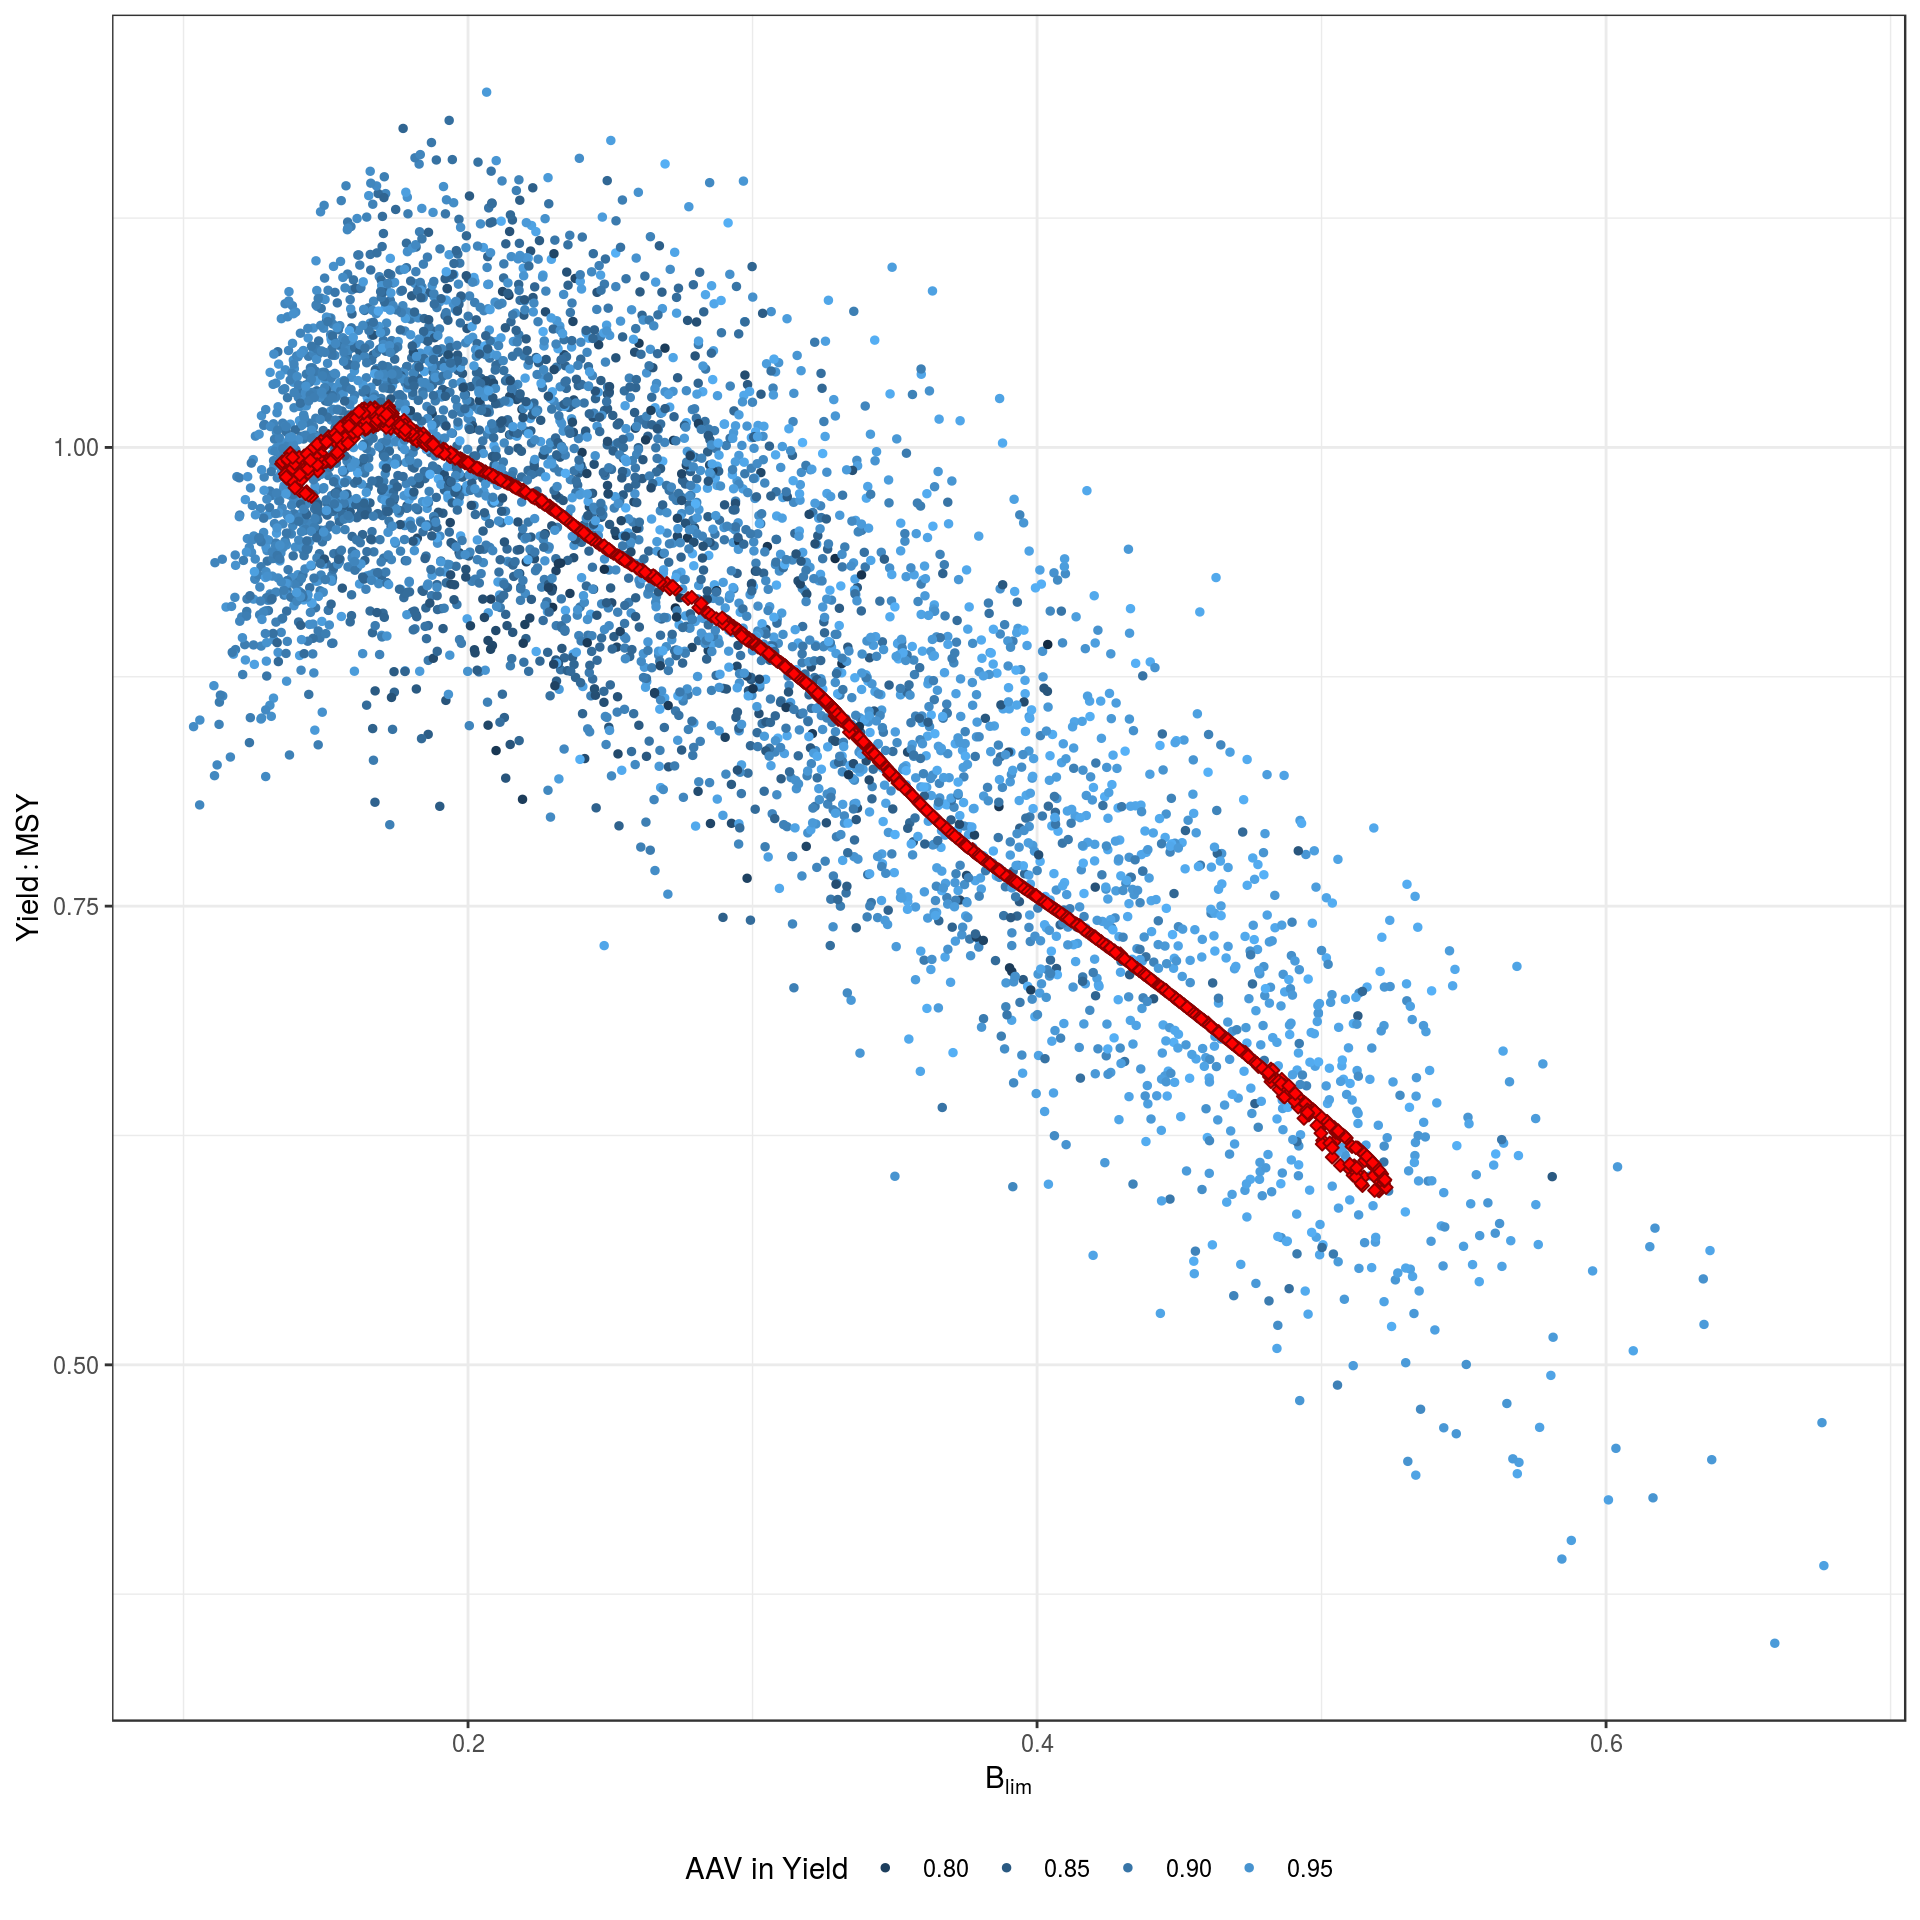
\includegraphics[width=\textwidth]{base-figScatter2-1.png}
\caption{Pareto frontier, showing  the trade-off between yield (Yield:MSY) and the average SSB relative to  are shown for the individual management strategy evaluations (blue) along with the pareto frontier (red).}
\label{fig:pareto}
\end{figure}

\newpage
\begin{figure}[h]
\centering
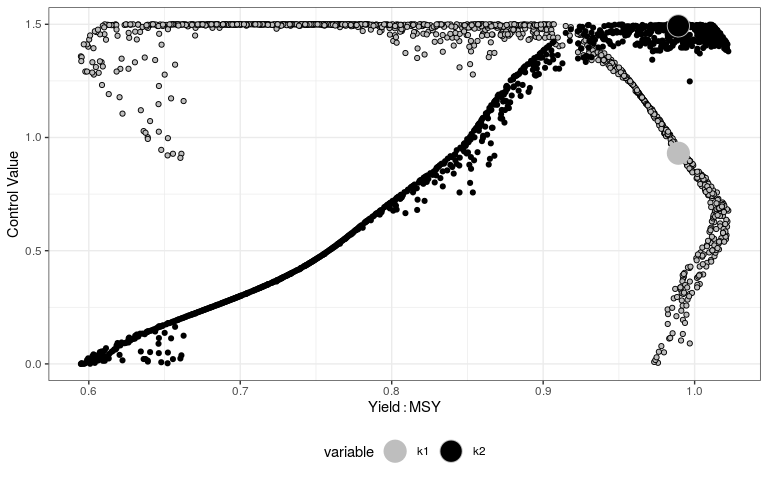
\includegraphics[width=\textwidth]{figs-figYield-1.png}
\caption{Calibration regression values for the control parameters K1 and K2 for the pareto frontier for , large point is for safety~0.7.}
\label{fig:control}
\end{figure}

\newpage
\begin{figure}[h]
\centering
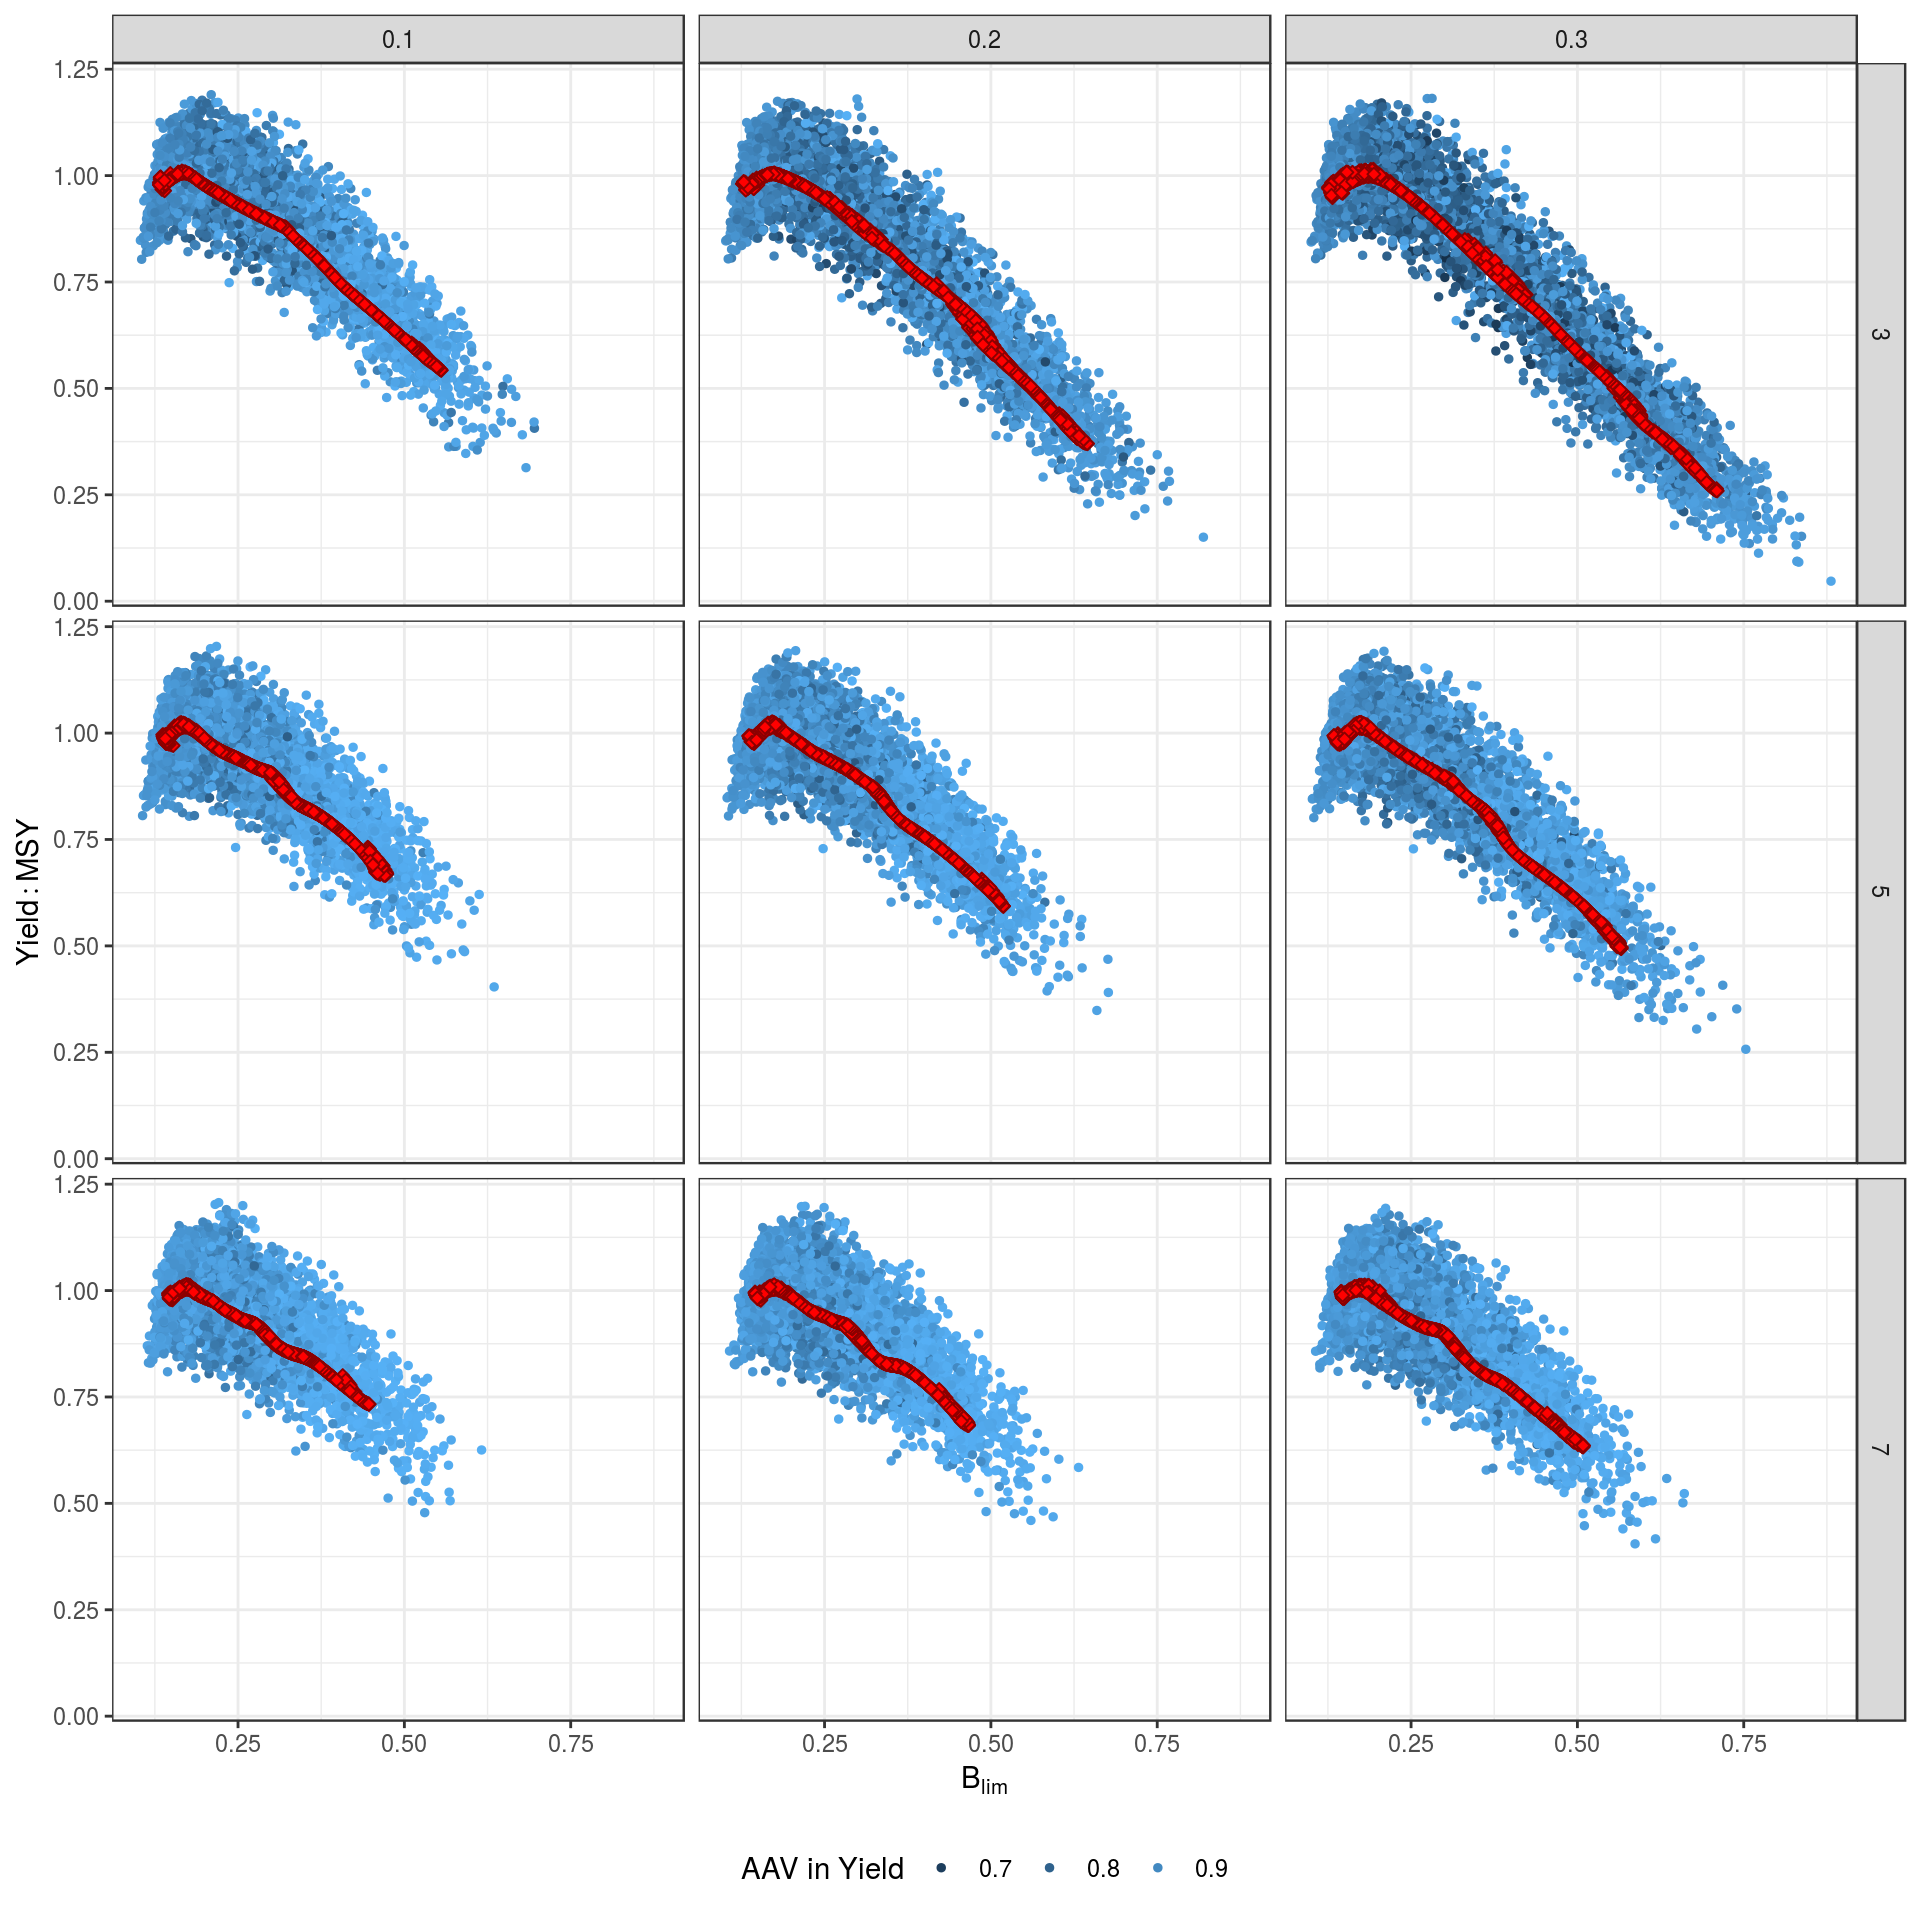
\includegraphics[width=\textwidth]{scenarios-unnamed-chunk-4-1.png}
\caption{Pareto frontier.}
\label{fig:voi}
\end{figure}

\newpage
\begin{figure}[h]
\centering
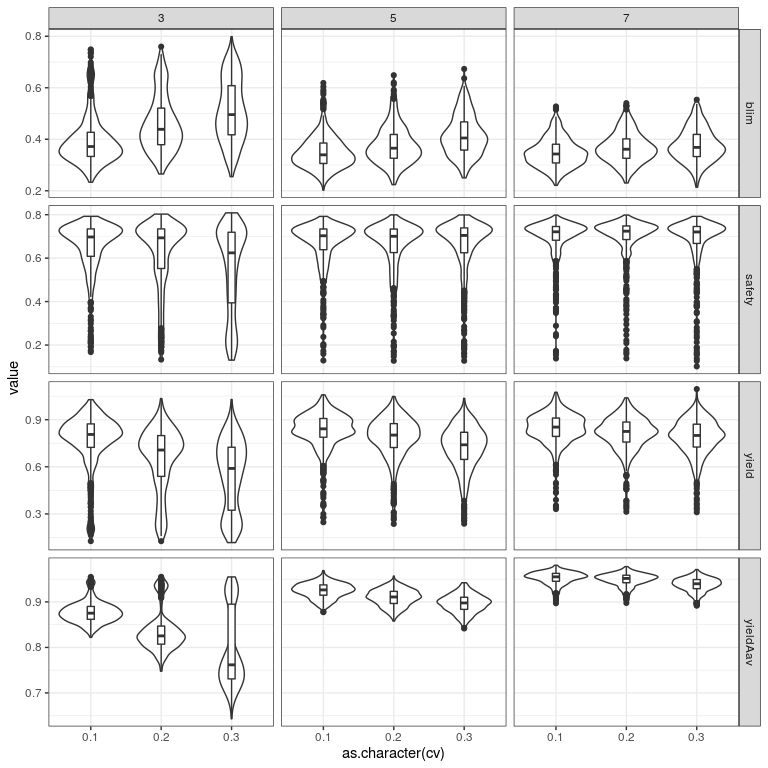
\includegraphics[width=\textwidth]{figs-unnamed-chunk-1-1.png}
\caption{.}
\label{fig:mse}
\end{figure}


\clearpage
\section{Appendix}


2012a. ICES Implementation of Advice for Data-limited Stocks in 2012 in its 2012 Advice. ICES CM 2012/ACOM 68: 42 pp.

ICES. 2017a. Report of the ICES Workshop on the Development of Quantitative Assessment Methodologies based on Life-history traits, exploitation characteristics, and other relevant parameters for data-limited stocks in categories 3-6 (WKLIFE VI), 3-7 October 2016, Lisb. ICES CM 2016/ACOM:59: 106 pp.


\end{document}


